\documentclass[10pt]{beamer}

\usepackage[T2A]{fontenc}
\usepackage[utf8]{inputenc}
\usepackage[russian,english]{babel}

\usefonttheme[onlymath]{serif}

\usetheme[progressbar=frametitle]{metropolis}
\usepackage{appendixnumberbeamer}

\usepackage{booktabs}
\usepackage[scale=2]{ccicons}

\usepackage{pgfplots}
\usepgfplotslibrary{dateplot}

\usepackage{xspace}
\newcommand{\themename}{\textbf{\textsc{metropolis}}\xspace}
\newcommand{\TODO}[1]{\textbf{\textcolor{red}{TODO: #1}}}

\date{}
\author{Екатерина Тузова}


\title{Лекция 6}
\subtitle{Перцептрон}

\begin{document}

\maketitle

\section{Разбор летучки}

\section{Мотивирующий пример}

{\foot{\href{https://www.kaggle.com/c/dogs-vs-cats}{Dogs vs. Cats}}
\begin{frame}{Пример}
  \centering
  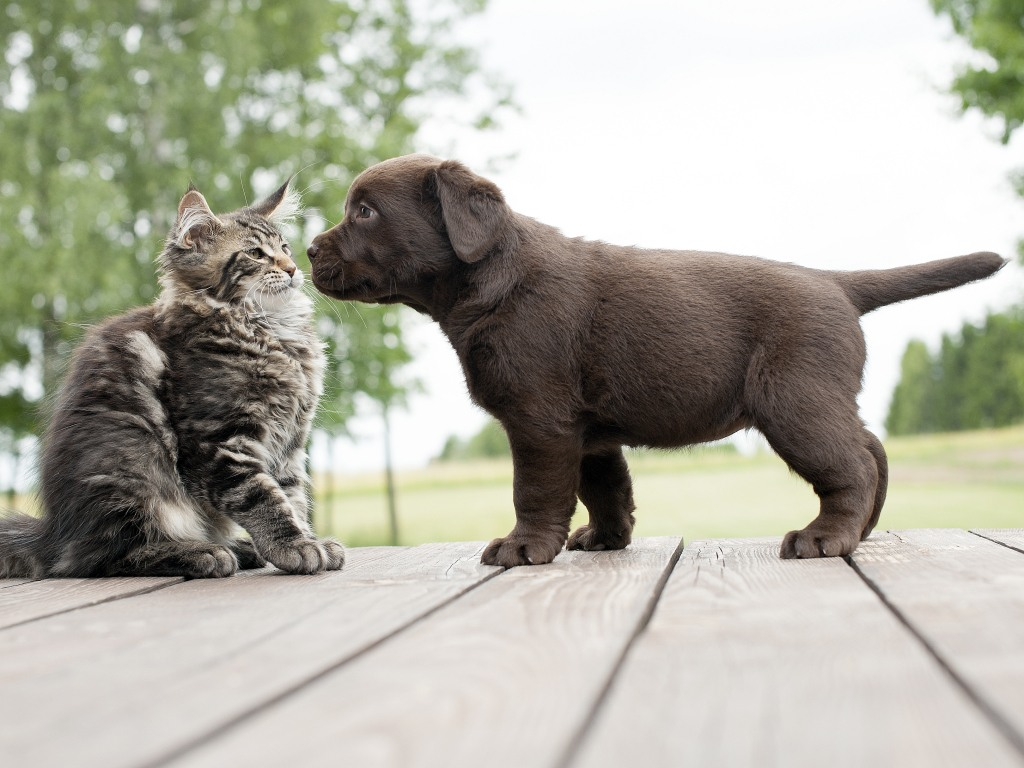
\includegraphics[width=0.9 \textwidth, keepaspectratio]{images/catvsdog}
\end{frame}
}

{\foot{\href{https://www.kaggle.com/c/dogs-vs-cats}{Dogs vs. Cats}}
\begin{frame}{Пример}
  \centering
  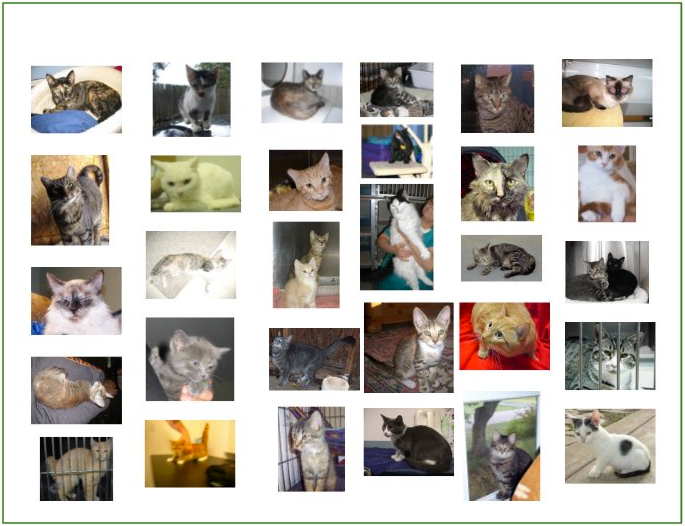
\includegraphics[width=0.9 \textwidth, keepaspectratio]{images/cats}
\end{frame}
}

{\foot{\href{https://www.kaggle.com/c/dogs-vs-cats}{Dogs vs. Cats}}
\begin{frame}{Пример}
  \centering
  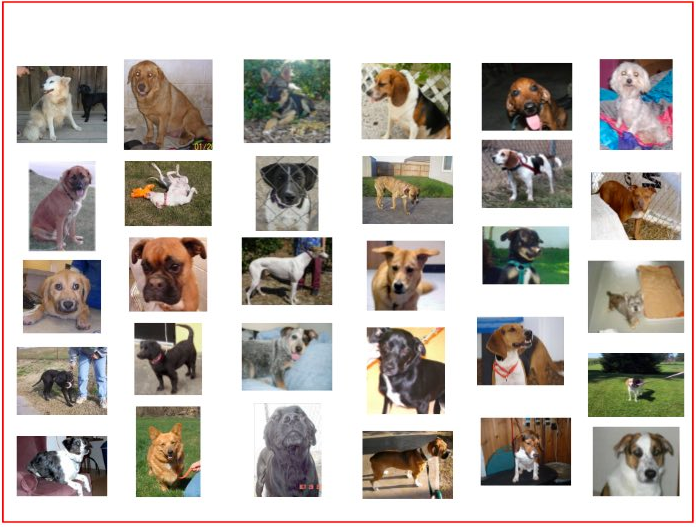
\includegraphics[width=0.9 \textwidth, keepaspectratio]{images/dogs}
\end{frame}
}

\begin{frame}{Постановка задачи}
  $X = \mathbb{R}^n$, ${Y = \left\{ -1, + 1\right\}}$\\
  ${X^l = (x_i, y_i)_{i = 1}^l}$ -- обучающая выборка\\
  \bigbreak
  \alert{Задача}: Построить алгоритм ${a \colon X \rightarrow Y}$, способный классифицировать произвольный объект ${x \in X}$.\\
  
\end{frame}

{\foot{decision surface, decision boundary}
\begin{frame}\frametitle{Перцептрон}
  \alert{Идея}: Назначим каждому признаку объекта некоторый вес. Посчитаем взвешенную сумму и если она больше некоторого порогового значения, отнесем объект к искомому классу. \\
  \bigbreak \pause
  Получается, что на самом деле мы ищем разделяющую поверхность.
\end{frame}
}

\begin{frame}{Пример}
  \centering
  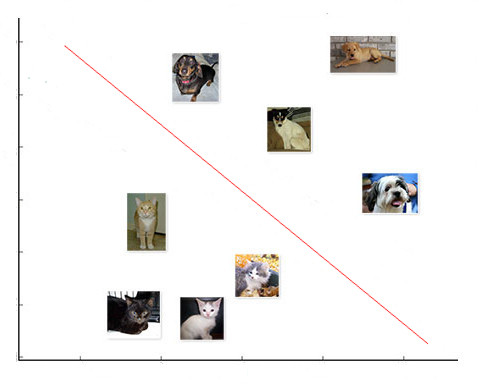
\includegraphics[width=0.9 \textwidth, keepaspectratio]{images/catdog1}
\end{frame}

\begin{frame}{Постановка задачи}
  $X = \mathbb{R}^n$, ${Y = \left\{ -1, + 1\right\}}$\\
  ${X^l = (x_i, y_i)_{i = 1}^l}$ -- обучающая выборка\\
  \bigbreak
  \alert{Задача}:\\
  $(n-1)$-мерную гиперплоскость, которая разделяет данные.
\end{frame}

\begin{frame}\frametitle{Модель McCulloch-Pitts}
  $X = \mathbb{R}^n$, ${Y = \left\{ -1, + 1\right\}}$\\
	\pause
	$$a(x,w) = \sigma(\sum\limits_{j=1}^n w_j x^j - w_0) = \sigma(\langle w, x \rangle)$$\\
  $x^j$ — числовые признаки, $j = 1,\dots, n$ \\	
	$w_j \in R$ -- веса признаков\\
	$\sigma(s)$ -- функция активации (например, $\sign$)
	\pause
	\begin{figure}[htbp]
	  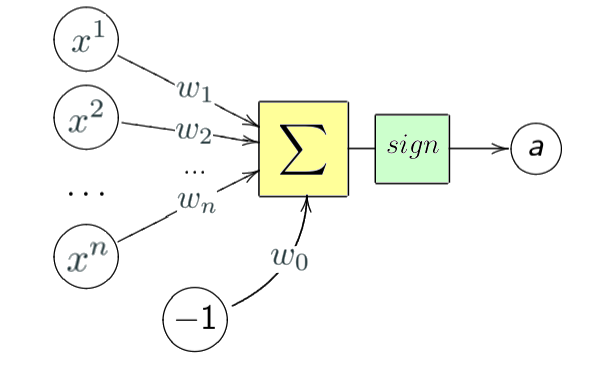
\includegraphics[height=100pt, keepaspectratio = true]{images/neuron-scheme}   
	\end{figure}
\end{frame}

\section{Как подобрать веса $w$?}

\begin{frame}
  \alert{Идея}: Хотелось бы минимизировать число неправильно классифицированных объектов.
\end{frame}

\begin{frame}{Алгоритм}
	\begin{algorithmic}[1]
        \Function{perceptron}{$X$}
            \State Инициализировать ${w_0, \dots, w_n}$
            \MRepeat [пока $w$ изменяются] 
               \For {$i = 1, \dots, l$}
                 \If {$a(x_i) \neq y_i$}
                   \State $w = w + y_i x_i$
                 \EndIf  
               \EndFor
           	\EndRepeat
        \EndFunction
    \end{algorithmic}
\end{frame}

\section{Что делать в случае нескольких классов?}

\begin{frame}
  \alert{Идея}: Для каждого класса заведём отдельный вектор $w_y$.
  \bigbreak \pause
  $$a(x) = \arg\max\limits_{y} w_y x $$
\end{frame}

\begin{frame}{Алгоритм}
	\begin{algorithmic}[1]
        \Function{multiclass\_perceptron}{$X$}
            \State Инициализировать ${w_0, \dots, w_n}$
            \MRepeat [пока $w$ изменяются] 
               \For {$i = 1, \dots, l$}
                 \State $a(x_i) = \arg\max\limits_{y} w_y x$                 
                 \If {$a(x_i) \neq y_i$}
                   \State $w_y = w_y - x_i$
                   \State $w_{y^{*}} = w_{y^{*}} + x_i$
                 \EndIf  
               \EndFor
           	\EndRepeat
        \EndFunction
    \end{algorithmic}
\end{frame}

\begin{frame} {Наблюдения}
    \begin{itemize} [<+->]
      \item[+] Алгоритм гарантированно сходится, если обучающая выборка линейно разделима
      \bigbreak
      \item[--] Не работает в случае неразделимой выборки 
      \item[--] "Слишком правильные" предсказания добавляют штраф       
    \end{itemize}
\end{frame}

\section{Будем улучшать алгоритм}

\begin{frame}{Алгоритм}
	\begin{algorithmic}[1]
        \Function{multiclass\_perceptron}{$X$, $\eta$}
            \State Инициализировать ${w_0, \dots, w_n}$
            \MRepeat [пока $w$ изменяются] 
               \For {$i = 1, \dots, l$}
                 \State $a(x_i) = \arg\max\limits_{y} w_y x$                 
                 \If {$a(x_i) \neq y_i$}
                   \State $w_y = w_y - \alert{\eta} x_i$
                   \State $w_{y^{*}} = w_{y^{*}} + \alert{\eta} x_i$
                 \EndIf  
               \EndFor
           	\EndRepeat
        \EndFunction
    \end{algorithmic}
\end{frame}

\begin{frame}{Постановка задачи}
  $X = \mathbb{R}^n$, ${Y = \left\{ -1, + 1\right\}}$\\
  ${X^l = (x_i, y_i)_{i = 1}^l}$ -- обучающая выборка\\
  \bigbreak
  \alert{Задача}:\\
  $(n-1)$-мерную гиперплоскость, которая разделяет данные \alert{как можно лучше}.
  \bigbreak \pause
  Как можно лучше -- это как?
\end{frame}

\begin{frame}{Пример}
  \centering
  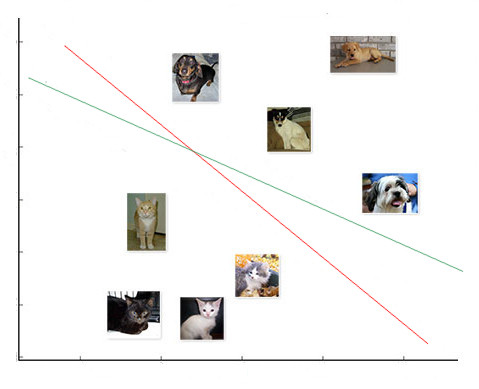
\includegraphics[width=0.9 \textwidth, keepaspectratio]{images/catdog}
\end{frame}

\begin{frame}{Постановка задачи}
  Как можно лучше:\\
  Два разделенных класса должны лежать как можно дальше от разделяющей гиперплоскости.
\end{frame}

\begin{frame}\frametitle{Определение отступа}
	${g = \langle \mathbf{w}, \mathbf{x}\rangle = 0}$ -- разделяющая поверхность\\
	$M_i(\mathbf{w}) = \langle \mathbf{w}, \mathbf{x_i}\rangle y_i$ -- отступ объекта $x_i$\\
	${M_i(\mathbf{w})<0}$ $\Rightarrow$ алгоритм $a(\mathbf{x},\mathbf{w})$ ошибается на $x_i$
\end{frame}

\begin{frame}\frametitle{Минимизация эмпирического риска}
	Число ошибок на обучающей выборке:\\
	\bigbreak
	${Q(\mathbf{w}) = \sum\limits_{i=1}^l \left[ M_i(\mathbf{w}) < 0 \right] \rightarrow \min\limits_{\mathbf{w}} }$\\
	\bigbreak
	${Q(\mathbf{w})}$ -- функционал качества\\
	\bigbreak
  \begin{itemize}
		\item[--] Индикаторную функцию сложно оптимизировать
		\item[--] Теряем информацию насколько ${i}$-й объект был надежен
	\end{itemize}
\end{frame}

\begin{frame}\frametitle{Отступ}
	\begin{figure}[htbp]
	  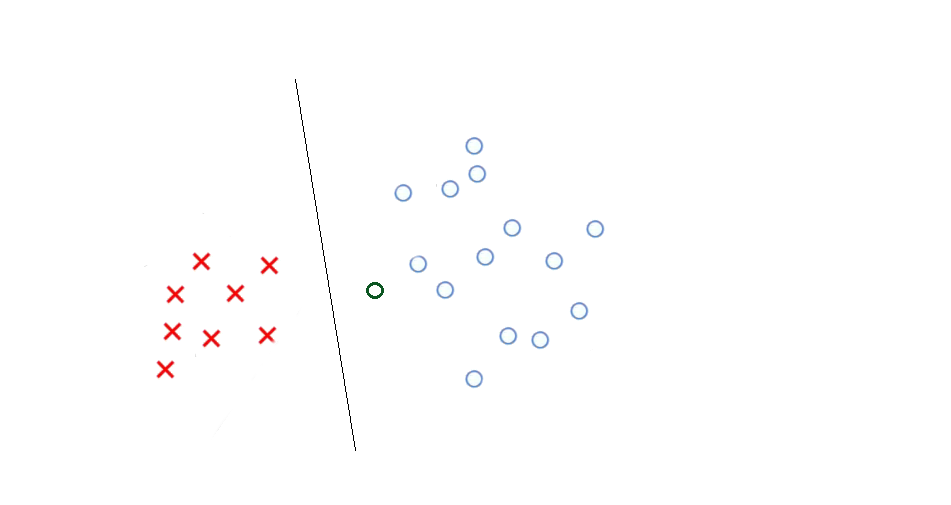
\includegraphics[height=190pt, keepaspectratio = true]{images/margin1}
	\end{figure}
\end{frame}

\begin{frame}\frametitle{Отступ}
	\begin{figure}[htbp]
	  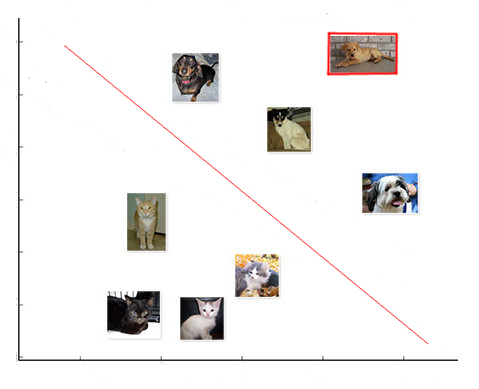
\includegraphics[height=190pt, keepaspectratio = true]{images/margin2}
	\end{figure}
\end{frame}

\begin{frame}\frametitle{Функция $[M<0]$}
	\begin{figure}[htbp]
	  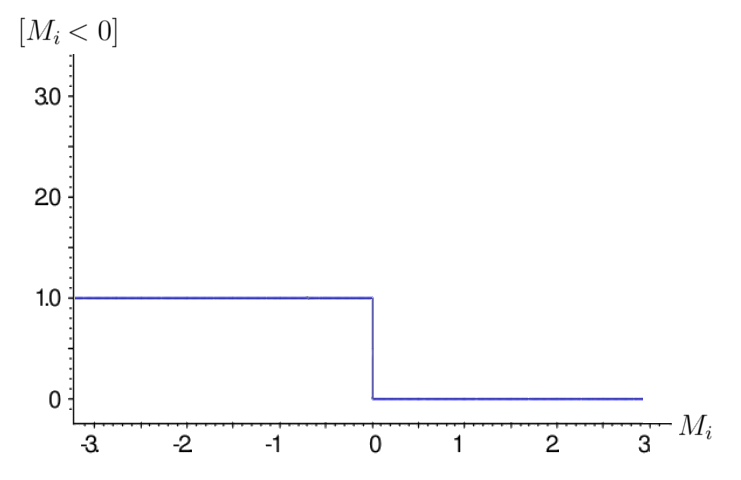
\includegraphics[height=160pt, keepaspectratio = true]{images/l1}
	\end{figure}
\end{frame}

\begin{frame}\frametitle{Минимизация эмпирического риска}
	${Q(\mathbf{w}) = \sum\limits_{i=1}^l \left[ M_i(\mathbf{w}) < 0 \right] \leq}$\\ \vspace{3mm}
	\hspace{10mm} ${\leq \sum\limits_{i=1}^l \mathcal{L}(M_i(\mathbf{w})) \rightarrow \min\limits_{\mathbf{w}} }$\\\vspace{3mm}
	$\mathcal{L}$ -- функция потерь, невозрастающая, неотрицательная.\\
	$\mathcal{L}$ должна мажорировать $\left[M_i(\mathbf{w}) < 0 \right]$
\end{frame}

\begin{frame}\frametitle{Примеры $\mathcal{L}$}
	\begin{figure}[htbp]
	  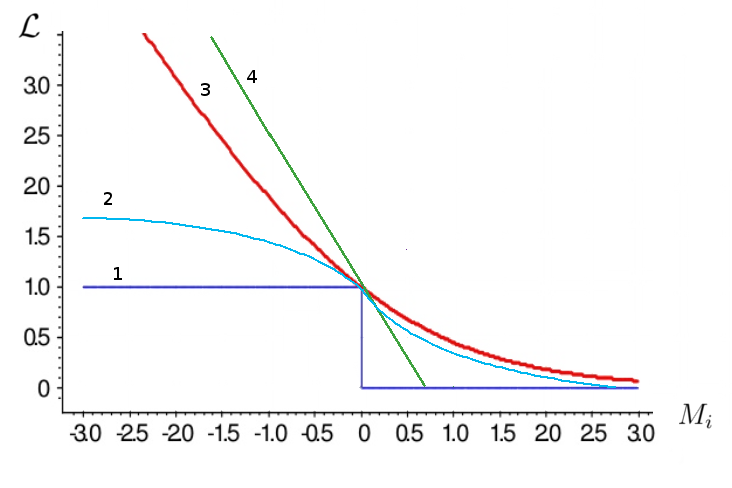
\includegraphics[height=160pt, keepaspectratio = true]{images/l}
	\end{figure}

	\begin{enumerate}
		\item $\left[M_i(\mathbf{w}) < 0 \right]$
		\item $S(M) = 2(1+e^M)^{-1}$ -- сигмоидная
		\item $L(M) = \log_2(1+e^{-M})$ -- логарифмическая
		\item $V(M) = (1-M)_+$ -- кусочно-линейная
	\end{enumerate}
\end{frame}

\section{Что такое градиент?}

\begin{frame}\frametitle{Градиент}
	\begin{figure}[htbp]
	  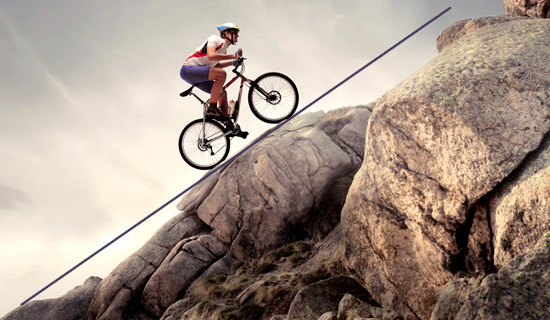
\includegraphics[height=160pt, keepaspectratio = true]{images/gradient}
	\end{figure}
\end{frame}

\begin{frame}\frametitle{Метод градиентного спуска}
	Input: $\alpha$ -- градиентный шаг (темп обучения)\\
	Output: $w_0, w_1, \dots, w_n$\\
	\vspace{3mm}
	Инициализировать: $w_j$, $j=0,\dots, n$\\
	Повторить пока $\mathbf{w}$ не стабилизируются:\\
	\hspace{10mm} $\mathbf{w} =  \mathbf{w} - \alpha \bigtriangledown Q(\mathbf{w})$\\
	
	\vspace{10mm}
	$\bigtriangledown Q(\mathbf{w}) = (\frac{\partial Q(\mathbf{w})}{\partial w_j})_{j=0}^n$\\
\end{frame}

\begin{frame}\frametitle{Градиентный спуск}
	\begin{figure}[htbp]
	  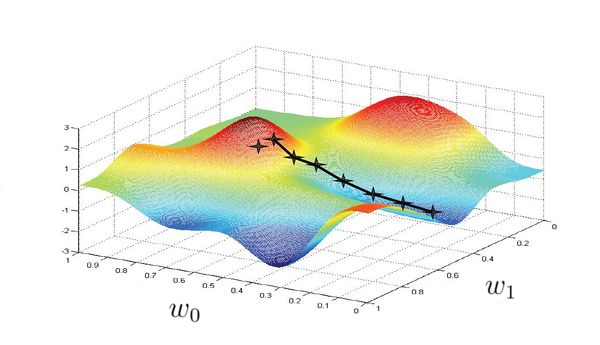
\includegraphics[height=160pt, keepaspectratio = true]{images/gradient_descent}
	\end{figure}
\end{frame}

\begin{frame}\frametitle{Метод градиентного спуска}
	Случай двух признаков.\\
	Input: $\alpha$ -- градиентный шаг (темп обучения)\\
	Output: $w_0, w_1$\\
	\vspace{3mm}
	Инициализировать: $w_0$, $w_1$\\
	Повторить пока $w_0$ и $w_1$ не стабилизируются:\\
	\hspace{10mm} $tmp_0 =  w_0 - \alpha \frac{\partial Q(w)}{\partial w_0}$\\
	\hspace{10mm} $tmp_1 =  w_1 - \alpha \frac{\partial Q(w)}{\partial w_1}$\\
	\hspace{10mm} $w_0 = tmp_0$\\
	\hspace{10mm} $w_1 = tmp_1$
\end{frame}

\section{Почему важно обновить $w_0$ и $w_1$ одновременно?}

\begin{frame}\frametitle{Градиент функционала качества $Q$}
	$$\bigtriangledown Q(\mathbf{w}) = (\frac{\partial Q(\mathbf{w})}{\partial w_j})_{j=0}^n = \sum\limits_{i=1}^l \mathcal{L}'(\langle \mathbf{w}, \mathbf{x_i} \rangle y_i) \mathbf{x_i} y_i$$\\
\end{frame}

\begin{frame}\frametitle{Маленький градиентный шаг}
	\begin{figure}[htbp]
	  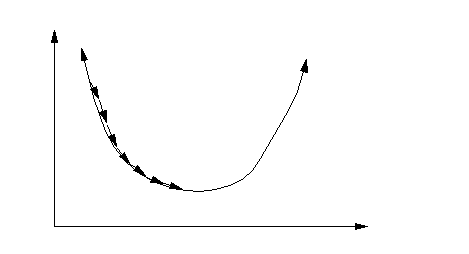
\includegraphics[height=160pt, keepaspectratio = true]{images/learning_rate_small}
	\end{figure}
\end{frame}

\begin{frame}\frametitle{Большой градиентный шаг}
	\begin{figure}[htbp]
	  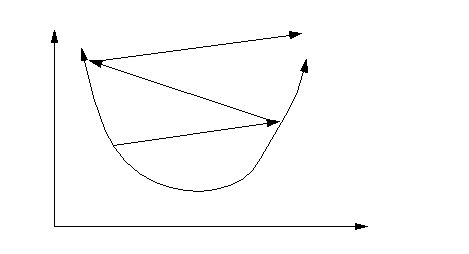
\includegraphics[height=160pt, keepaspectratio = true]{images/learning_rate_large}
	\end{figure}
\end{frame}

\begin{frame}\frametitle{Выбор величины шага}
	\begin{itemize}
		\item[--] $\alpha_t \rightarrow 0$\\
		\item[--] Метод скорейшего градиентного спуска:\\
		$Q(w - \alpha \bigtriangledown Q(w)) \rightarrow \min\limits_{\alpha}$
		\item[--] Пробные случайные шаги
	\end{itemize}
\end{frame}

\section{В чем проблема?}

\begin{frame}\frametitle{Метод стохастического градиента}
	$$\mathbf{w} =  \mathbf{w} - \alpha \sum\limits_{i=1}^l \mathcal{L}'(\langle \mathbf{w}, \mathbf{x_i}\rangle y_i)\mathbf{x_i}y_i$$\\
	\bigbreak \pause
	\alert{Идея}: Давайте брать $(x_i, y_i)$ по одному и сразу обновлять вектор весов
\end{frame}

\begin{frame}\frametitle{Алгоритм}
	Input: $X^l$, $\alpha$, $\eta$\\
	Output: $w_0, w_1, \dots, w_n$\\
	\vspace{3mm}
	Перемешать данные в $X^l$\\
	Инициализировать: $w_j$, $j=0,\dots, n$\\
	\hspace{35mm} ${Q}(\mathbf{w}) = \sum\limits_{i=1}^l \mathcal{L}(\langle \mathbf{w}, \mathbf{x_i} \rangle y_i)$\\
	Повторить пока $Q$ и/или $w$ не стабилизируются:\\
	\hspace{5mm} Взять $x_i$ из $X^l$\\
	\hspace{5mm} Потеря: $\varepsilon_i = \mathcal{L}(\langle \mathbf{w}, \mathbf{x_i} \rangle y_i)$\\
	\hspace{5mm} Градиентный шаг: $w =  w - \alpha \mathcal{L}'(\langle \mathbf{w}, \mathbf{x_i}\rangle y_i)\mathbf{x_i}y_i$\\
	\hspace{5mm} Оценить $Q = (1-\eta)Q + \eta \varepsilon_i$
\end{frame}

\begin{frame}\frametitle{Градиентный спуск}
	\begin{figure}[htbp]
	  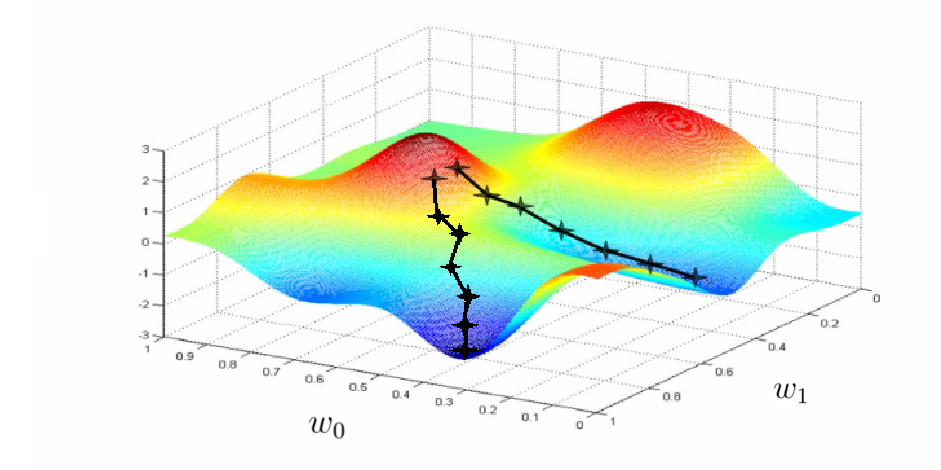
\includegraphics[height=160pt, keepaspectratio = true]{images/gradient_descent2}
	\end{figure}
\end{frame}

\begin{frame}\frametitle{Учет ошибки $\varepsilon_i$ в алгоритме}
	\begin{figure}[htbp]
	  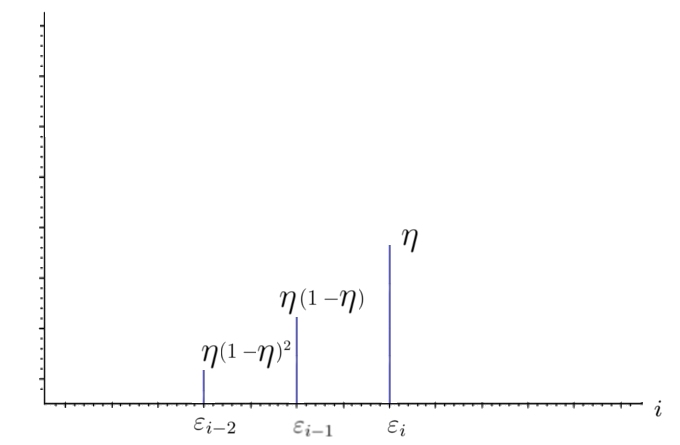
\includegraphics[height=160pt, keepaspectratio = true]{images/l2}
	\end{figure}
\end{frame}

\section{Что значит -- "пока $Q$ и/или $w$ не стабилизируются"?}

\begin{frame}\frametitle{Зависимость $Q$ от номера итерации}
	\begin{figure}[htbp]
	  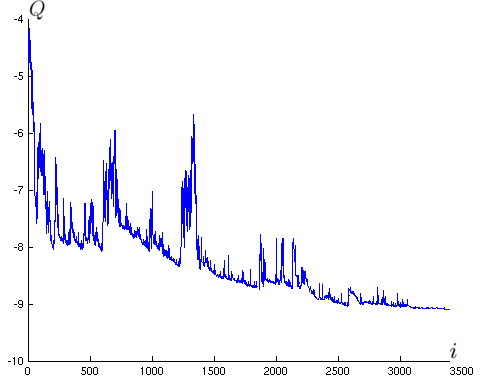
\includegraphics[height=160pt, keepaspectratio = true]{images/stochastic_gradient}
	\end{figure}
\end{frame}

\begin{frame}\frametitle{Зависимость $Q$ от номера итерации}
	\begin{figure}[htbp]
	  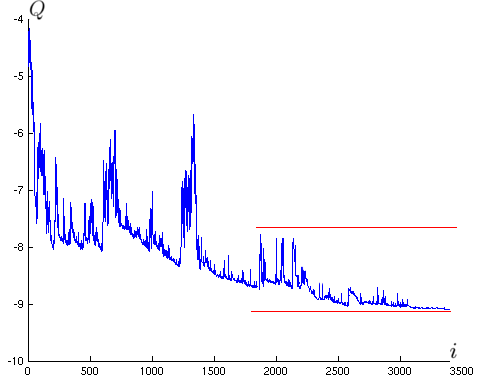
\includegraphics[height=160pt, keepaspectratio = true]{images/stochastic_gradient1}
	\end{figure}
\end{frame}

\begin{frame}\frametitle{Актуальные вопросы}
	\begin{itemize} [<+->]
		\item[--] Инициализация весов
		\item[--] Порядок предъявления объектов
	\end{itemize}
\end{frame}

\section{Инициализация весов}

\begin{frame}\frametitle{Инициализация весов}
	\begin{itemize}
		\item[--] $w_j = 0$, j = 1, \dots, n
		\item[--] $w_j = random(-\frac{1}{2n}, \frac{1}{2n})$ -- небольшие случайные значения
		\item[--] Обучение по небольшой случайной подвыборке объектов
		\item[--] Многократный запуск из разных случайных начальных приближений
	\end{itemize}
\end{frame}

\section{Порядок предъявления объектов}

\begin{frame}\frametitle{Порядок предъявления объектов}
	\begin{itemize}
		\item[--] Попеременно брать объекты из разных классов
		\item[--] Чаще брать те объекты, на которых была допущена большая ошибка
		\item[--] Вообще не брать "хорошие" объекты с $M_i > \mu_+$
		\item[--] Вообще не брать выбросы с $M_i < \mu_-$
	\end{itemize}
\end{frame}

\begin{frame}\frametitle{Плюсы и минусы}
	\begin{itemize} [<+->]
	\item[+] Легко реализовать
	\item[+] Легко обобщить на разные $g$, $\mathcal{L}$
	\item[+] Не обязательно брать все элементы выборки для обучения
	\bigbreak
	\item[--] Возможна медленная сходимость
	\item[--] Застревание в локальных минимумах
	\item[--] Подбор параметров
	\item[--] Проблема переобучения
	\end{itemize}
\end{frame}

\section{Почему случается переобучение?}

\begin{frame}\frametitle{Проблема переобучения}
	$a(\mathbf{x}, \mathbf{w}) = sign(\langle \mathbf{w}, \mathbf{x}\rangle)$\\
	Линейная зависимость признаков:\\
	$\forall \mathbf{x} \exists \mathbf{u}: \langle \mathbf{u}, \mathbf{x}\rangle = 0$\\
	$\Rightarrow \forall \gamma: a(\mathbf{x}, \mathbf{w}) = sign(\langle \mathbf{w} + \gamma \mathbf{u}, \mathbf{x}\rangle)$\\
	\bigbreak
	Алгоритм $a'$ работает точно также как исходный $a$.\\
	А значит мы можем получить любое решение из семейства $\mathbf{w} + \gamma \mathbf{u}$
\end{frame}

\begin{frame}\frametitle{Проблема переобучения}
	\begin{itemize}
		\item[--] Слишком мало объектов
		\item[--] Слишком много признаков
		\item[--] Линейная зависимость признаков
	\end{itemize}
\end{frame}

\begin{frame}\frametitle{Как заподозрить?}
	\begin{itemize}
		\item[--] Слишком большие веса $\Vert \mathbf{w} \Vert$
		\item[--] Неустойчивость $a(\mathbf{x},\mathbf{w})$
		\item[--] Плохое качество классификации на контрольных данных
	\end{itemize}
\end{frame}

\begin{frame}\frametitle{Решение}
	\begin{itemize}
		\item[--] Сокращение весов
		\item[--] Ранняя остановка алгоритма
	\end{itemize}
\end{frame}

\section{Как можно сокращать веса?}

\begin{frame}\frametitle{Сокращение весов}
	Штраф за увеличение нормы вектора весов:\\
	$Q_{\tau} = Q + \frac{\tau}{2}\Vert \mathbf{w} \Vert^2 \rightarrow \min\limits_{\mathbf{w}}$\\
	\bigbreak
	Градиент:\\
	$\bigtriangledown Q_{\tau} = \bigtriangledown Q + \tau \mathbf{w}$\\
	\bigbreak
	Градиентный шаг:\\
	$\mathbf{w} = \mathbf{w}(1-\alpha \tau) - \alpha \bigtriangledown Q(\mathbf{w})$\\
	$\tau$ -- параметр регуляризации
\end{frame}

\section{Как подобрать $\tau$?}

\section{Степени свободы}

\begin{frame}\frametitle{Степени свободы}
	\begin{itemize}
		\item[--] Вид разделяющей поверхности
		\item[--] Вид аппроксимации функционала качества $Q(\mathbf{w})$
		\item[--] Вид регуляризатора
	\end{itemize}
\end{frame}

\begin{frame}[standout]
  Вопросы?
\end{frame}

\appendix

\begin{frame}\frametitle{На следующей лекции}
	\begin{itemize}
    	\item[--] Функционалы качества
    	\item[--] Неравенство Хефдинга
    	\item[--] Близость гипотез
    	\item[--] Неравенство Вапника-Червоненкиса
    	\item[--] Генерация модельных данных    	    	
	\end{itemize}
\end{frame}
\end{document}

\end{document}